\section{Benchmarking}
\label{sec:benchmarking}

We now evaluate generic properties of the presented I/O processing
schemes.
To do so, we remove constraints of I/O devices, and focus on naive
microbenchmarking programs of matrix operations performing with the host
and the device memory.
In particular, timing analysis of addition and multiplication of varying
sized matrices is conducted.
These programs are considered as the most basic parallel computing
programs also used in prior work~\cite{Rossbach_SOSP11}.
Since our focus is on data access and I/O processing, but not on
computation, we choose matrix addition as a microbenchmark, as it is 
a straightforward operation for the GPU.
Matrix multiplication, on the other hand, is also included to briefly
illustrate how an increase of computational complexity and data accesses
affects time to completion.
We also showcase effective host read and write throughput for each I/O
processing scheme.
This benchmarking clarifies the capabilities of the presented scheme, not
specific to plasma control but applicable to generic low-latency
GPU computing.

The microbenchmarking experiments are conducted using the NVIDIA Quadro
5000 GPU (448 cores and 2.5GB memory), which is more end-user oriented
than the Tesla C2050 used in the case study.
Note that the supported number of compute cores is the same between
these two GPUs.

\subsection{Matrix Operations}
\label{sec:matrix}

We first demonstrate performance details of matrix operations.
To highlight the details, we use a large size of $2048\times2048$ matrix
in this experiment.
The properties of operations focused on are listed as follows:

\begin{itemize} \itemsep1pt
 \item {\bf Init:} GPU initialization time.
 \item {\bf MemAlloc:} Memory allocation time, with respect to the host
       and/or the device memory.
 \item {\bf DataInit:} Matrix initialization time.
 \item {\bf HtoD:} Copy time from the host to the device memory (only \hd).
 \item {\bf Exec:} Execution time of the kernel function.
 \item {\bf DtoH:} Copy time from the device to the host memory (only
       \hd\ and \dmh).
 \item {\bf DataRead:} Access time to read the result.
 \item {\bf Close:} Context destroying time.
\end{itemize}

\begin{figure}[t]
\centering
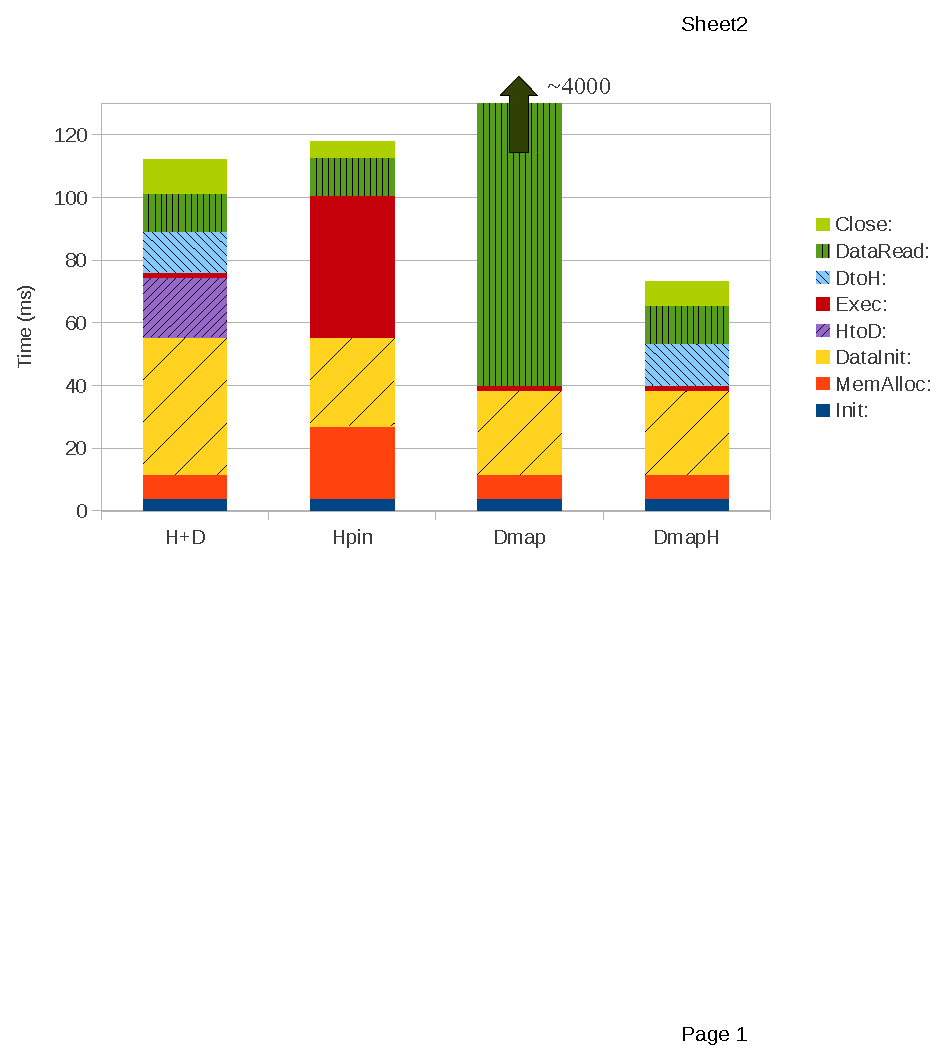
\includegraphics[width=0.5\textwidth, trim=0.0in 3.25in 0.0in 0.25in,
 clip=true]{eps/madd_time_spent.eps}
\caption{Details of matrix addition.}
\label{fig:madd_time_spent}
\end{figure}
\begin{figure}[t]
\centering
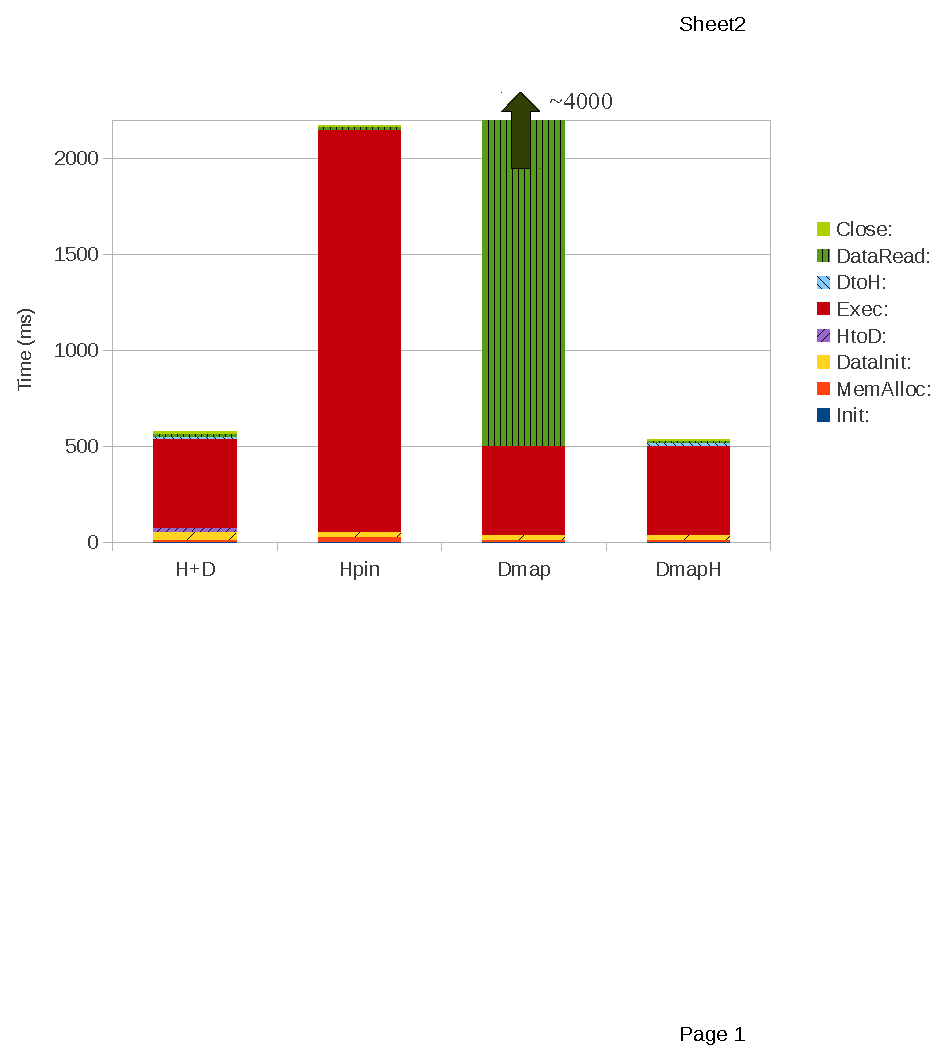
\includegraphics[width=0.5\textwidth, trim=0.0in 3.0in 0.0in 0.5in,
 clip=true]{eps/mmul_time_spent.eps}
\caption{Details of matrix multiplication.}
\label{fig:mmul_time_spent}
\end{figure}
\begin{figure}[t]
\centering
\includegraphics[width=0.5\textwidth, trim=0.0in 2.0in -0.3in 0.74in,
 clip=true]{eps/madd_time.eps}
\caption{Total matrix addition times.}
\label{fig:madd_time}
\end{figure}
\begin{figure}[t]
\centering
\includegraphics[width=0.5\textwidth, trim=0.0in 2.0in -0.3in 0.72in,
 clip=true]{eps/mmul_time.eps}
\caption{Total matrix multiplication times.}
\label{fig:mmul_time}
\end{figure}

Figure \ref{fig:madd_time_spent} shows where the system spends its time
in performing a $2048\times2048$ integer matrix addition using each of
the four schemes.
First, it is clear from Figure \ref{fig:madd_time_spent} that using our
{\dmh} scheme the total time to completion is less than the others, 
almost $34\%$ less than its nearest competitor, \textit{i.e.}, the {\hd}
scheme.

A more interesting observation is the comparison of how much
time is spent for each sub-task.
For most time categories, the {\dmh} scheme seems to enjoy the best of
each of the other three.
The memory allocation time for the {\dmh} scheme is nearly
identical to that of the {\hd} and the {\dm} schemes, and clearly less
than the {\hp} scheme.
The same is true for the execution times. 
Similarly, for data initialization, the {\dmh} scheme is just as good as
the {\hp} and the {\dm} scheme, which are superior to the {\hd} scheme.

The most notable difference among the four schemes is the data read time
for the {\dm} scheme, which is orders-of-magnitude greater than the
rest.
A $2048\times2048$ integer matrix represents 16MB of data, and the {\dm}
scheme reads 4 bytes at a time across the PCIe bus.
This was the motivation for our \dmh\ scheme.
Instead of reading one matrix element at a time, the {\dmh} scheme first
copies the data to the host before reading.
This evinces that the {\dm} scheme may suffer from a large size of data,
while it was very effective for the case study presented in
Section~\ref{sec:case_study} that deals with 96 inputs and 64 outputs of
16-bit data, \textit{i.e.}, 2KB of data.

The same anomaly is present in the execution time for the {\hp} scheme
-- the GPU must read one element at a time from the host memory, while
in the other three schemes the data reside on the GPU during
computation.
This makes the {\hp} scheme increasingly inferior as the data size
grows.

Figure \ref{fig:mmul_time_spent} shows the same time analysis for matrix
multiplication.
The only difference appears in the execution times.
This is not surprising as the multiplication experiments are exactly the
same as the addition ones except for the kernel function on the GPU.
In fact, if execution times are omitted, Figures
\ref{fig:madd_time_spent} and \ref{fig:mmul_time_spent} would look
almost identical.
This observation implies that the zero-copy I/O processing schemes are
not really appreciated by strongly compute-intensive applications.

While the above experiments do present a real-world scenario, in a
real-time system it is more likely that tasks are performed repeatedly,
and therefore the GPU initialization and closing costs might occur only
once -- the same context loaded a priori would remain active while only
the data might change.
In addition, it could be the case that the memory allocated for the task
could be reused, and only the contents modified.
For these reasons, the remainder of our analysis focuses only on read,
write, transfer, and execution. 

Figure~\ref{fig:madd_time} shows the time to completion of matrix
addition as a function of matrix size at the logarithmic scale.
The {\hp} scheme appears to be the best performer until a matrix size of
$32\times32$, corresponding to a data size of 4KB for each matrix, at
which point the {\dmh} becomes superior.
This is also reflected in the matrix multiplication times, as shown in
Figure~\ref{fig:mmul_time}. 
One thing to note is the growth rate of the {\hp} in matrix
multiplication; since each thread must perform multiplication and
addition $n^2$ times, as compared with one addition in matrix addition,
the number of reads that occur across the PCIe bus increases by a
greater exponential factor.
We expect that the time for the {\hp} scheme would eventually surpass
the {\dm} scheme, as the trend in the graph indicates.

%Note that even with the logarithmic time scale the curves appear exponential because while the matrix length and width increase as $2^n$ the data size of the
%matrix is $2^n \times 2^n \times 4 =  2^{2n+2}$ bytes (for 32-bit integers).

\subsection{Data Throughput}
\label{sec:data_throughput}

Finally, we evaluate the data throughput of the presented I/O processing
schemes, independent of computational units.
In other words, this evaluation shows the pure performance of data
communication between the host and the device memory.
We use the term ``effective throughput'' to mean ($size/time$) where
$time$ is measured from the beginning of data initialization to the
point at which it is actually available to the GPU.
For example, in the case of the {\hd} scheme, this corresponds to the
total time for the host processor to write to each element in the data
structure, which is in the host memory, plus the time to copy the data
to the device memory.

Figure~\ref{fig:write_tput} shows that the write throughput of the
{\dmh} is better than the {\hd} scheme by about a factor of 2 and at
least as good as the others, which all coincide almost exactly in the
graph.
Meanwhile, Figure~\ref{fig:read_tput} paints a slightly different
picture for read throughput.
It should not be surprising that the {\hp} scheme outperforms the rest
as it represents the host iterating over a data structure that is
already in the host memory.
The {\hd} and the {\dmh} schemes, on the other hand, must first copy the
data from the device to the host memory, and they achieve roughly equal
performance.
Note that they coincide in the graph.
Finally, the {\dm} scheme is the weakest performer due to a large
number of small reads that occur across the PCIe bus.

\begin{figure}[t]
\centering
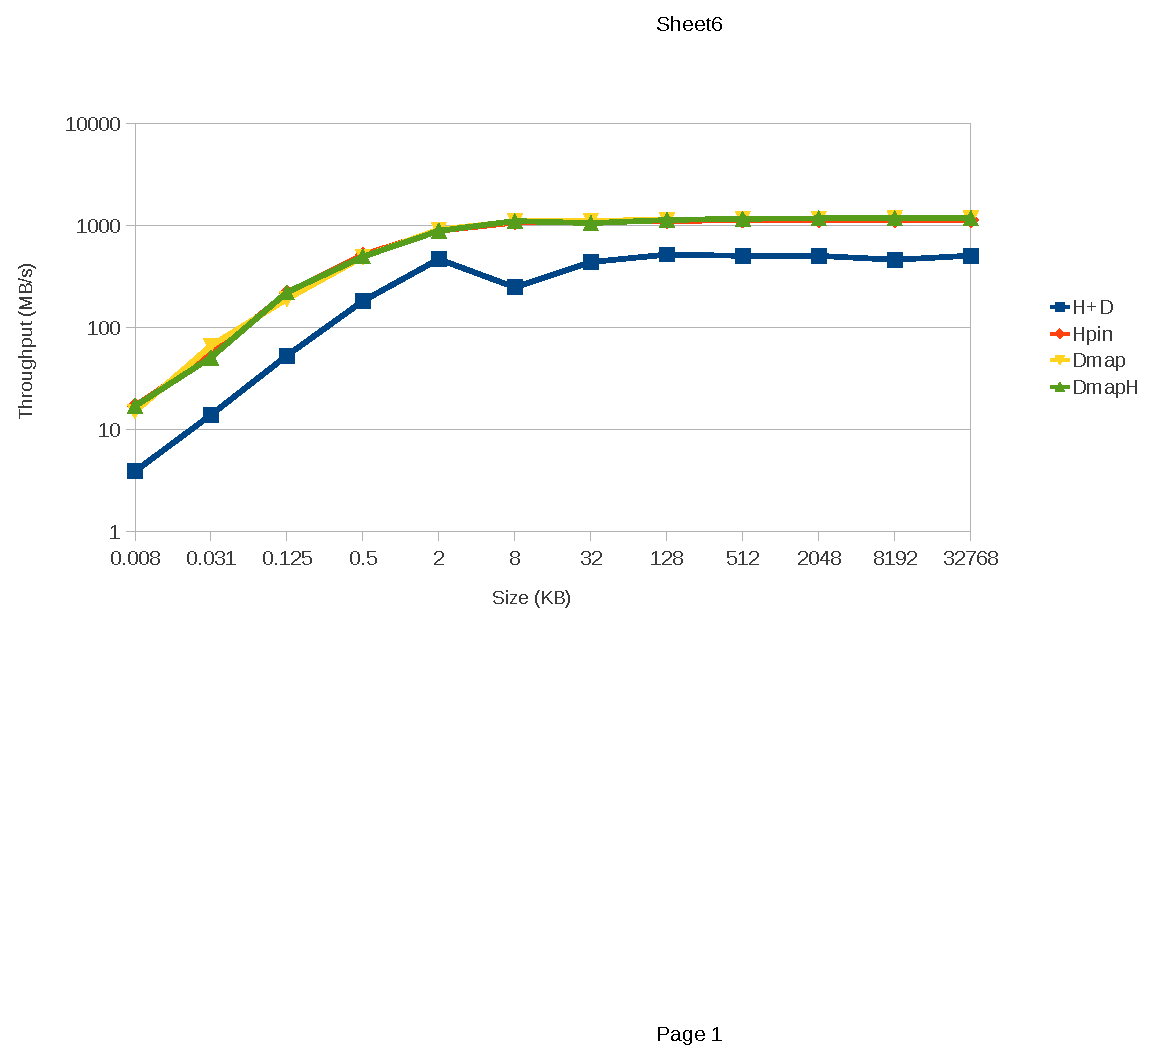
\includegraphics[width=0.5\textwidth, trim=0.0in 2.75in -0.1in 0.60in,
 clip=true]{eps/write_tput.eps}
\caption{Host write throughput.}
\label{fig:write_tput}
\end{figure}
\begin{figure}[t]
 \centering
 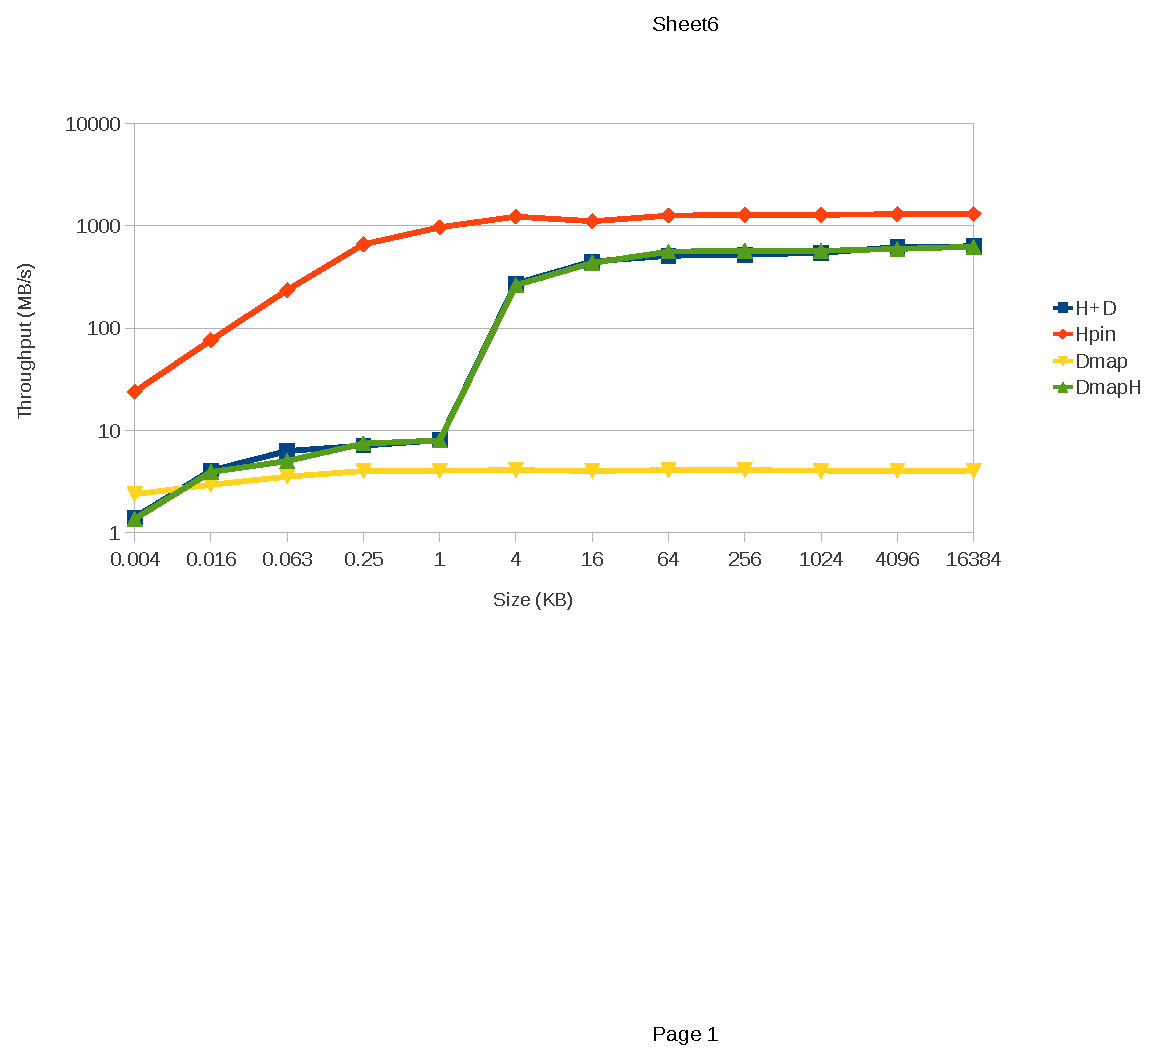
\includegraphics[width=0.5\textwidth, trim=0.0in 2.5in -0.1in 0.6in,
 clip=true]{eps/read_tput.eps}
 \vspace{-2em}
 \caption{Host read throughput.}
\label{fig:read_tput}
\end{figure}
